\documentclass[12pt]{article}
\usepackage{fullpage}
\usepackage{graphicx}
\usepackage{amsmath}
\usepackage{amssymb}
\usepackage{mathtools}
\usepackage[]{mcode}
\usepackage{booktabs,caption}

\DeclareMathOperator{\Tr}{Tr}
\DeclareMathOperator*{\argmin}{arg\,min}
\DeclareMathOperator{\mcx}{\mathcal{X}}
\begin{document}

{\parindent 0pt \begin{tabular}[t]{l}
CE263N \\
\end{tabular}  \hfill \today \vskip 0.2in }

\parindent 0pt
\parskip 8pt

\begin{center}
\large\bf Homework \#1 \\
\large\bf Name: \textnormal{Ian Bolliger}\\
\large\bf Student ID: \textnormal{25939428}\\
\end{center}

\bigskip

\section{}
	\begin{itemize}
		\item I found an average time of clustering 100K samples into 100 clusters to be 2.1s for vanilla k-means, and 1.2s for MiniBatch k-means. Both algorithms were being run with only 1 set of initialization points. This choice was made because the procedure for using multiple initializations varies across the two algorithms. In vanilla k-means, the entire algorithm is run to convergence for each set of centroid seeds. In MiniBatch k-means, only the inertia of those centroid seeds are calculated (using a specified batch size to calculate this); then, only the best initialization is chosen and run through the algorithm. In order to compare the two algorithm's speeds on a level playing field, only a single initialization set was used.
		
		\item Because of changes in the implementation of these algorithms there were no issues with memory size at high $k$. However, MiniBatch k-means did not converge in under 1.5 hrs for 90k clusters. Thus, if your criteria for a successful implementation of an algorithm is that it can run in that timeframe, an estimate of $k_{max}$ is 70-90k. MiniBatch k-means began to increase in processing time rapidly around $k=25,000$, surpassing the processing time of vanilla k-means. A sample of algorithm processing times is included in Table \ref{tab:title}.
		
		\item Two regions of $\epsilon$ were found that generated approximately 100 clusters with $MinPts = 100$. This behavior is explained through the following: At the lower $\epsilon$ values, many points are classified as outliers and thus only around 100 clusters can be formed. As we increase $\epsilon$, more groups of outlier points can become clusters, and $n_clusters$ increases. Eventually, as $\epsilon$ further increases, more and more of these distinct clusters are merged and $n_clusters$ begins to decrease again. Thus, I observed ranges of $\epsilon_{100}$ of $[489-492m]$ and $[1003-1020m]$. In the smaller $\epsilon$ range, the processing time was roughly 1.3s; in the larger range, it was roughly 2.1s.
	\end{itemize}
\begin{minipage}\linewidth
    \centering	
    \captionof{table}{Processing Time for Both k-means Algorithms (s)} \label{tab:title} 
    \begin{tabular}{lrr}
    
    \toprule
    k &  k-means & MiniBatch k-means \\
    \midrule
    1     &     0.02 &              0.11 \\
    100   &     2.05 &              1.22 \\
    1024  &    26.13 &              9.49 \\
    10539 &   250.84 &             80.46 \\
    89794 & 1,504.24 &               Did Not Converge \\
    \bottomrule
    \end{tabular}
\end{minipage}

\section{}

	\begin{figure}[H]
		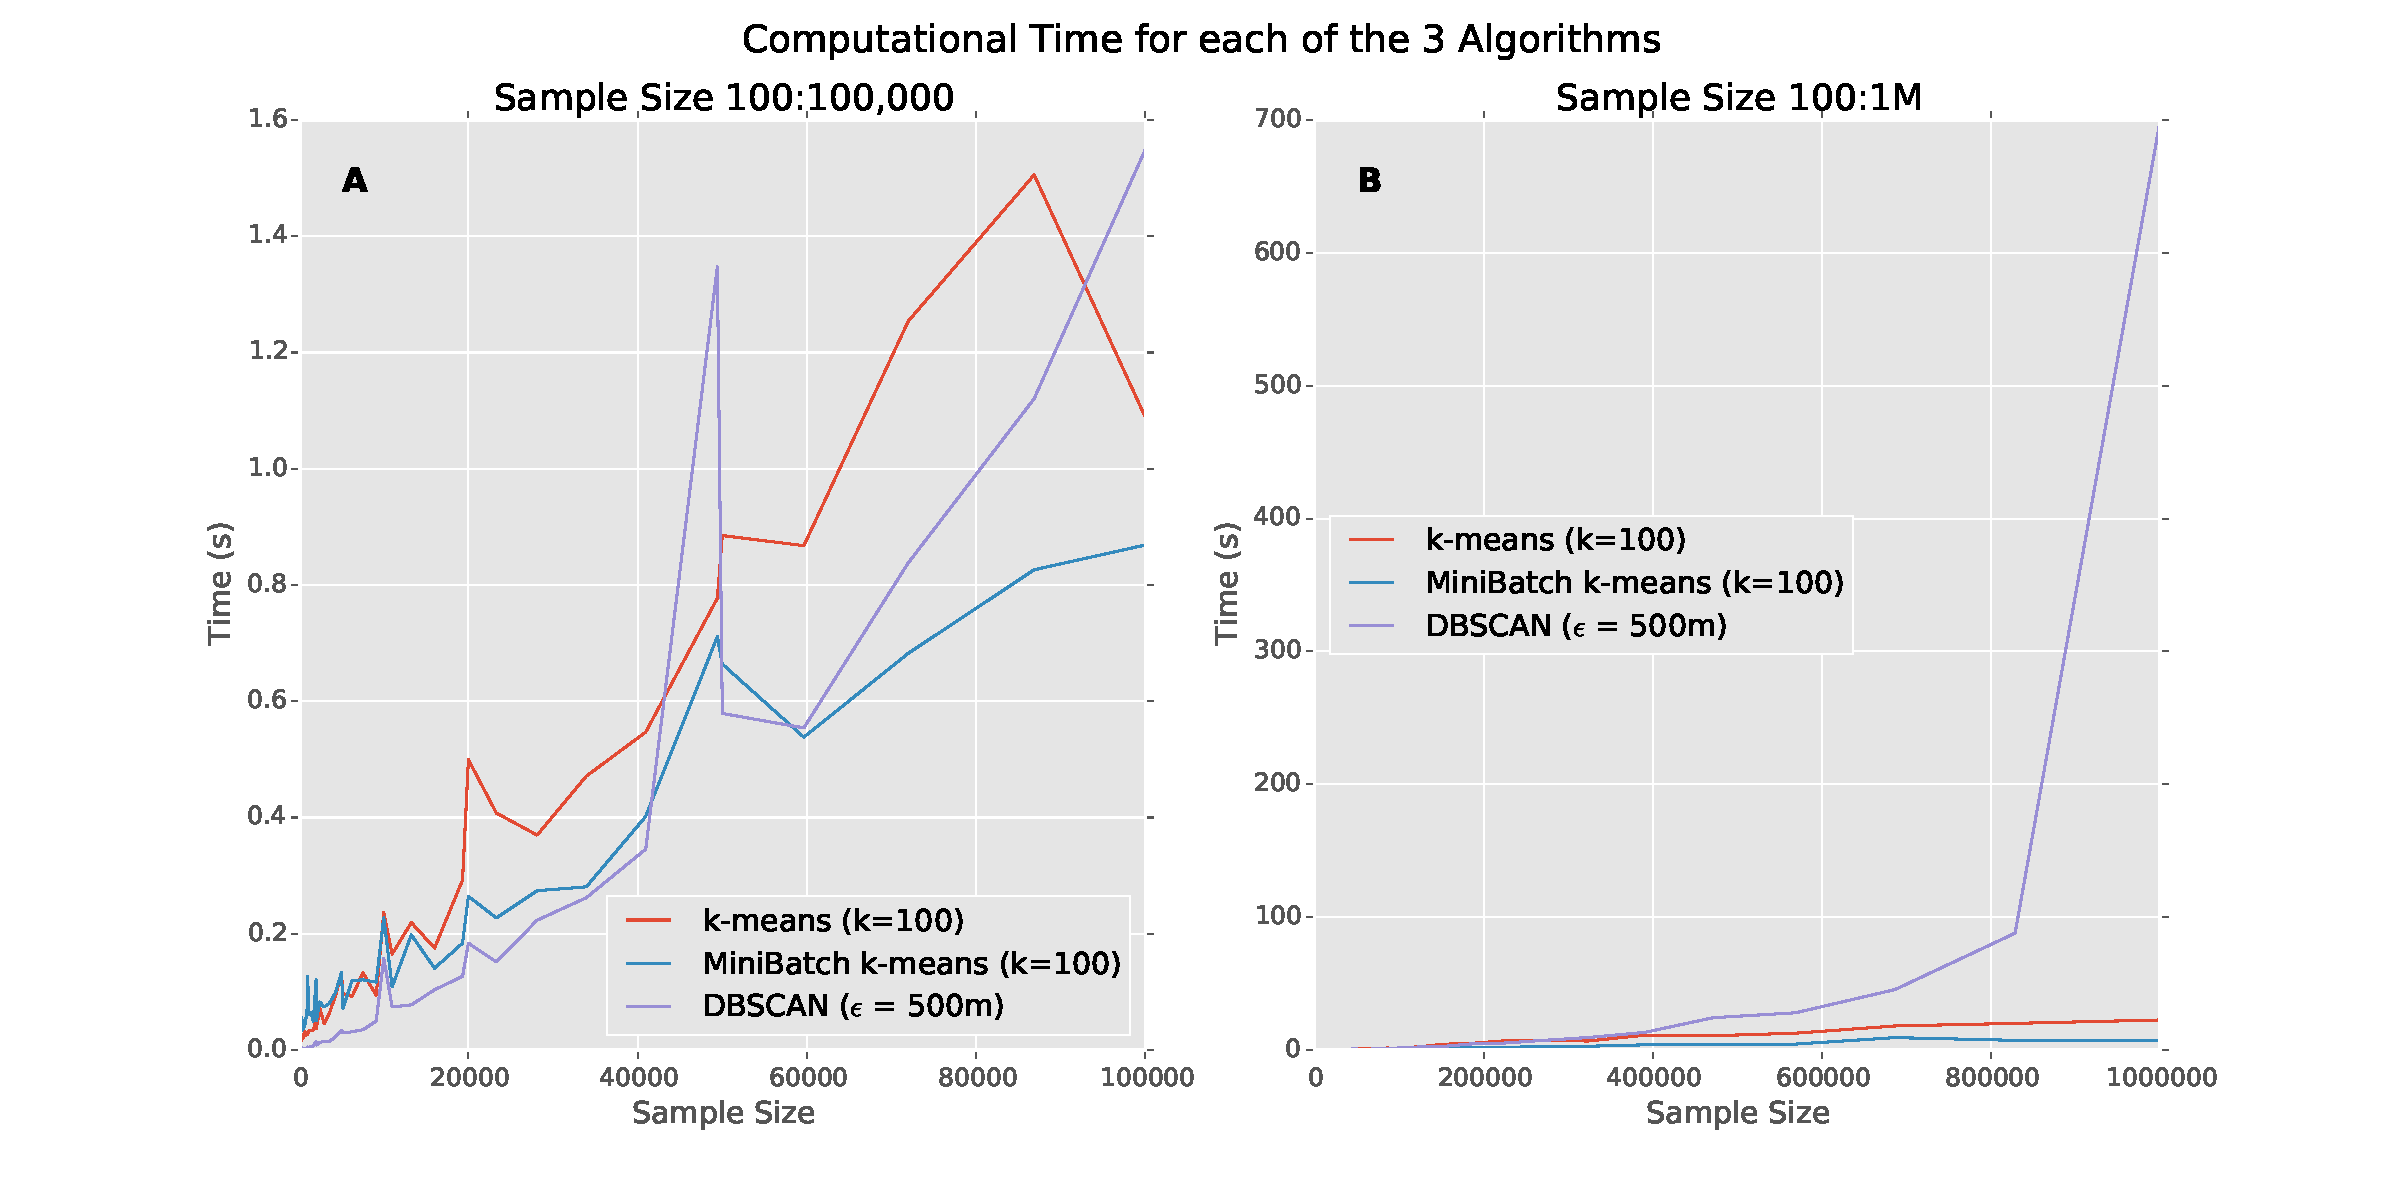
\includegraphics[width=7.5in]{comptime}
		\centering
		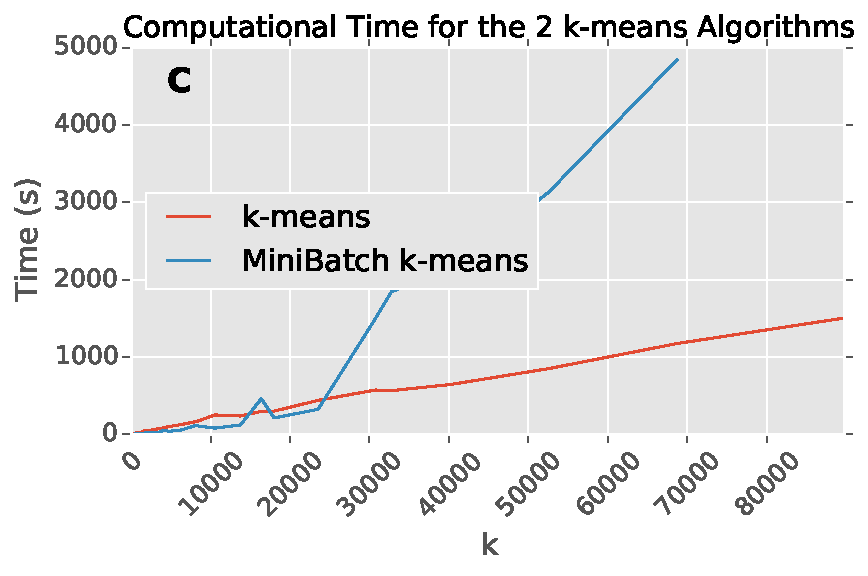
\includegraphics[width=3.75in,]{comptime_k}
		\caption{Processing Times for the various algorithms as functions of (a,b) sample size and (c) number of clusters.} \label{figs}
	\end{figure}
	
	Because I was able to run each method on the full 1M tweets, estimation of the processing times are not needed. Table \ref{tab2:title} describes the times for each algorithm. Note that $\epsilon=500m$ and $MinPts = 100$ for the DBSCAN runs, and a batch size of 10k ($1\%$ of the data) was used for MiniBatch. Again, only 1 centroid seed was used for both k-means algorithms. Figure \ref{figs} displays representative processing times on my machine.
	
\begin{minipage}\linewidth
    \centering	
    \captionof{table}{Processing Time for Each Algorithm on the full dataset (s)} \label{tab2:title} 
	\begin{tabular}{lrrrr}
    \toprule
    k-means & MiniBatch k-means &      DBSCAN &  DBSCAN n\_clusters \\
    \midrule
    23 &              7.3 &  700 &                544 \\
    \bottomrule
    \end{tabular}
    \end{minipage}
    
\section{}
	As can be seen in Figure \ref{figs}b, DBSCAN processing times begin to increase rapidly around 300k. Thus, it seems reasonable that a 2-step clustering algorithm, in which MiniBatch k-means is run for $k=3$ or $4$ is a good place to start when looking for a computationally efficient clustering strategy. Running with fewer "step-1" clusters would lead to greater sample sizes (>300k) input into DBSCAN and exponentially greater processing times for "step-2". Running with a greater number of step-1 clusters (assuming serial architecture) would increase the number of times that DBSCAN must run but decrease the time of each run. In practice, it appears that anything from $k=1$ to $k=11$ has a relatively similar runtime for the overall algorithm (Figure \ref{times_2step}). At $k$ values over 11, the effect of having to run DBSCAN on additional clusters (and of having to generate more clusters from the initial MiniBatch k-means clustering) overcomes the effect of the algorithm being run on smaller subsets. As can be seen in Table \ref{tab3:title}, there does not appear to be any efficiency advantage to running a 3-step clustering algorithm, where two levels of MiniBatch k-means are followed by DBSCAN. As can also be seen in Table \ref{tab3:title}, the number of clusters identified increases with lower "step-1" clusters. If we truly wish to identify all of the clusters with 100 tweets within 100m of a point, then using fewer "step-1" clusters should be preferable. Thus, $k=3$ optimizes the skill of the overall algorithm within the constraint of being a near-efficient computational method.
	
	NOTE: Code is submitted separately as a .pdf of a notebook. Initial setup and loading of data occurs at the top, and the code specific to Part 3 is located under the section labeled "Part 3".
	
	\begin{figure}[H]
		\centering
		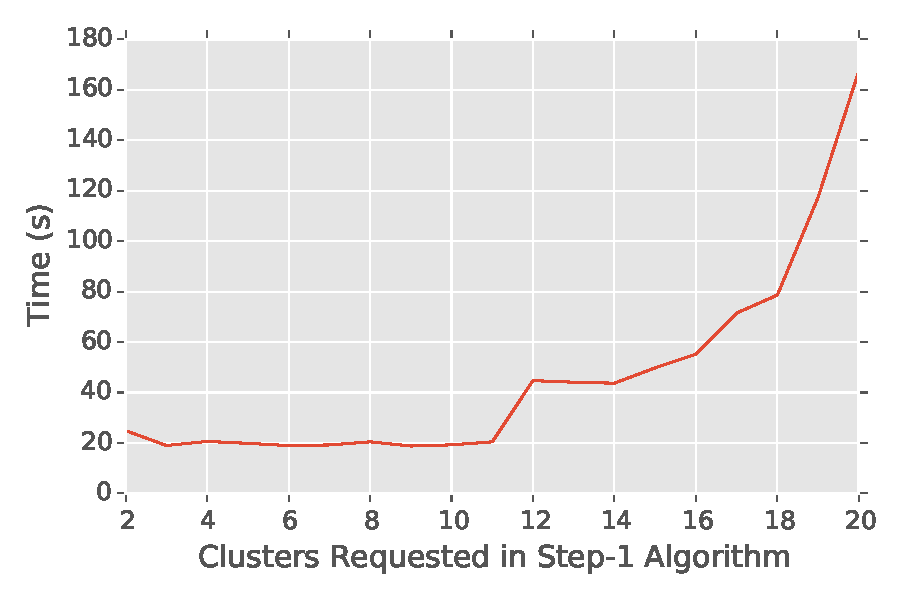
\includegraphics[width=3.75in]{2steptimes}
		\caption{Processing Times for the 2-step algorithm in which DBSCAN is run separately on "step-1" initially identified by a MiniBatch k-means algorithm.} \label{times_2step}
	\end{figure}
	
\begin{minipage}\linewidth
\centering
\captionof{table}{Processing Time for a 3-step Clustering Algorithm} \label{tab3:title} 
\begin{tabular}{llll}
\toprule
 k1 & k2  &      time & n\_clusters \\
\midrule
2  & 2 &  25.9 &       1589 \\
  & 3 &  28.4 &       1589 \\
  & 4 &  25.0 &       1589 \\
  & 5 &  25.3 &       1589 \\
 & 6 &  25.9 &       1589 \\
3  & 2 &  20.0 &       1398 \\
  & 3 &  20.7 &       1398 \\
  & 4 &  21.3 &       1398 \\
  & 5 &  21.7 &       1398 \\
 & 6 &  24.9 &       1398 \\
4  & 2 &  20.9 &       1361 \\
  & 3 &  22.1 &       1361 \\
  & 4 &  24.0 &       1361 \\
  & 5 &  23.8 &       1361 \\
 & 6 &  25.2 &       1361 \\
5  & 2 &  21.7 &       1349 \\
  & 3 &   23.1 &       1349 \\
  & 4 &  24.3 &       1349 \\
  & 5 &  25.5 &       1349 \\
 & 6 &  27.3 &       1349 \\
6  & 2 &  22.0 &       1263 \\
  & 3 &  23.8 &       1263 \\
  & 4 &  25.1 &       1263 \\
  & 5 &  28.7 &       1263 \\
  & 6 &  30.2 &       1263 \\
\bottomrule
\end{tabular}
\end{minipage}

\section{Extra Credit}
It's clear from the map contained in Figure \ref{map} that the cluster with the most tweets belongs to downtown San Francisco. Since that area is so dense, the area still forms a cluster even though people are tweeting about a wide range of topics. A quick visual analysis of the tweet texts did not help identify the cluster other than that many were about San Francisco. To confine the tweets further (to Downtown SF), plotting on the map was necessary. Code for generating this map can be found in the attached notebook.
	\begin{figure}[h]
		\centering
		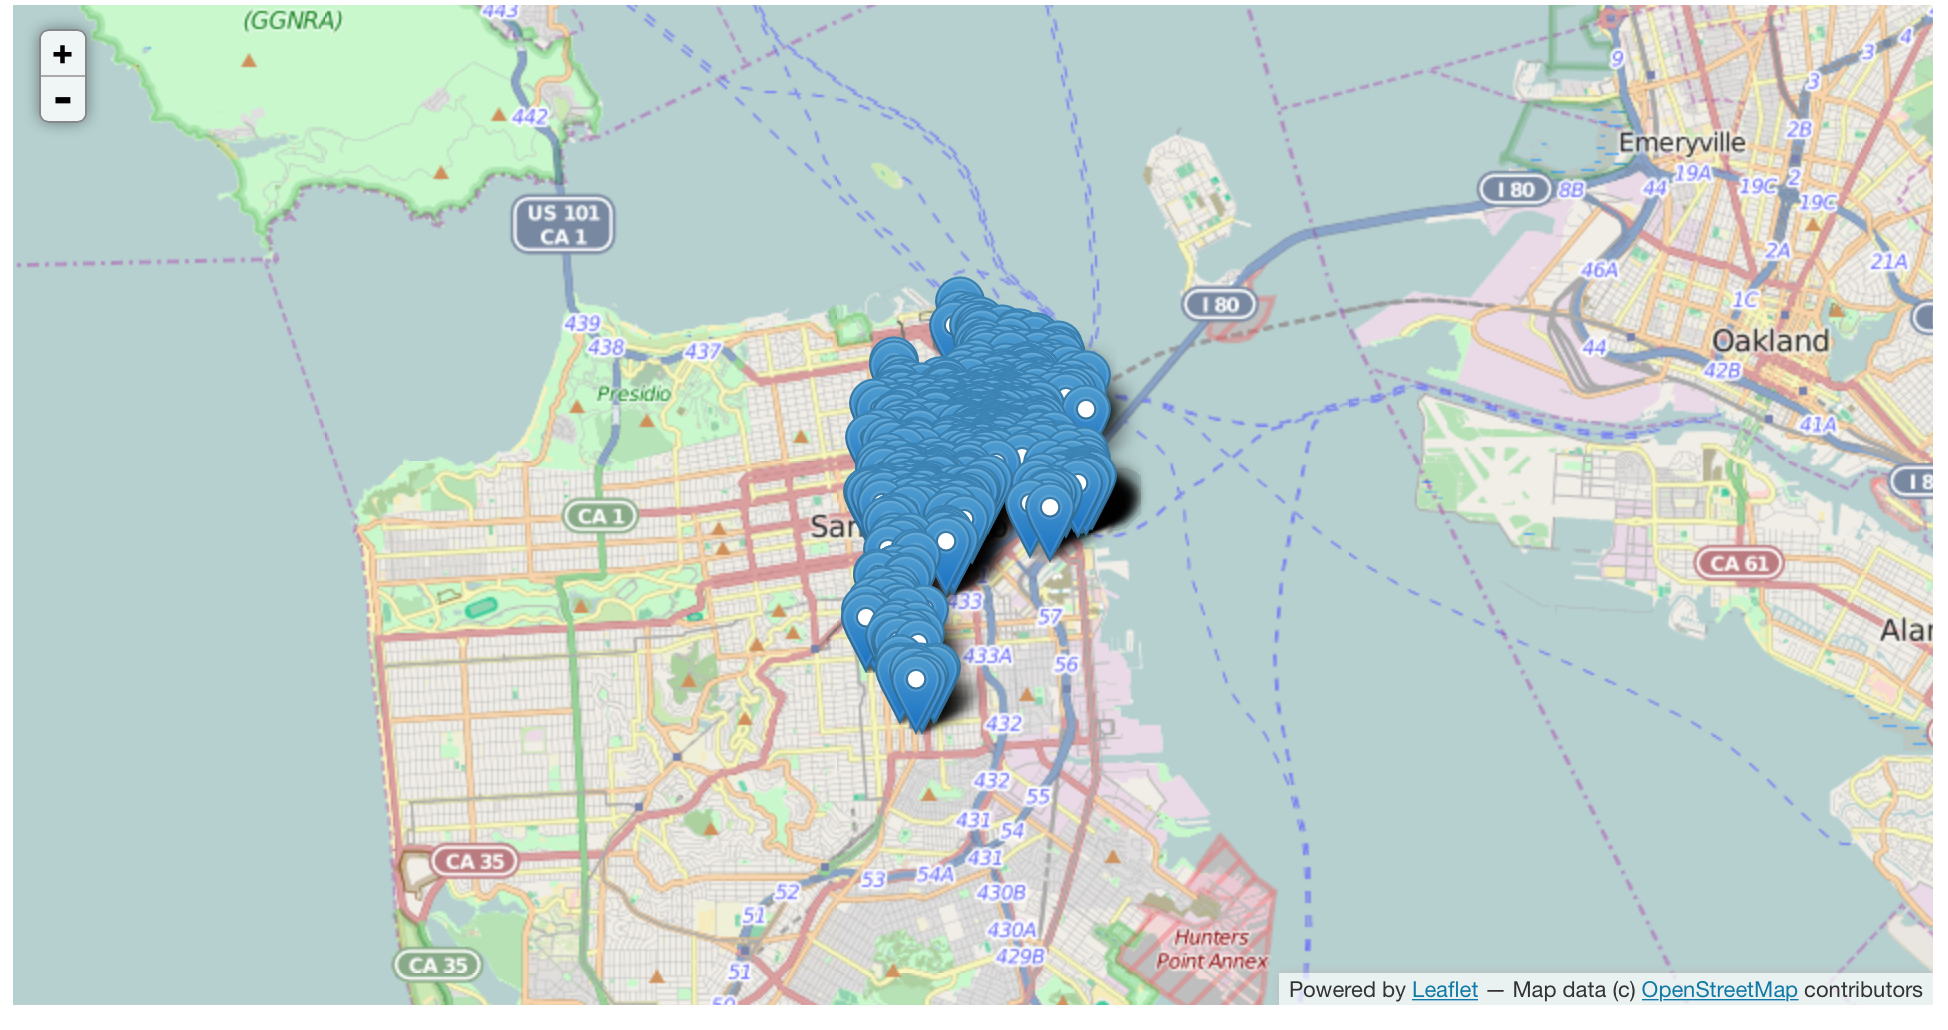
\includegraphics[width=6in]{map}
		\caption{Map of the largest cluster identified, which happens to be located in downtown SF.} \label{map}
	\end{figure}

\end{document}